\section{A Synchronous Channel}

We  now implement a simple synchronous channel---similar to that in
earlier chapters---using semaphores.  We  need three signals for each
message, in the following order:
%
\begin{enumerate}
\item The sender  signals to the receiver that it has deposited a value, on
  semaphore |slotFull|.

\item The receiver  signals back to the sender on semaphore |continue|,
  thereby providing a synchronisation.

\item The sender signals to the sender on the next round that the slot has
  been emptied, on semaphore |slotEmptied|.
\end{enumerate}
%
%These three semaphores will collectively provide mutual exclusion.
Figure~\ref{fig:semaphore-syncChan-SD} illustrates the sequence of signals. 

%%%%%

\begin{figure}[hbtp]
\begin{center}
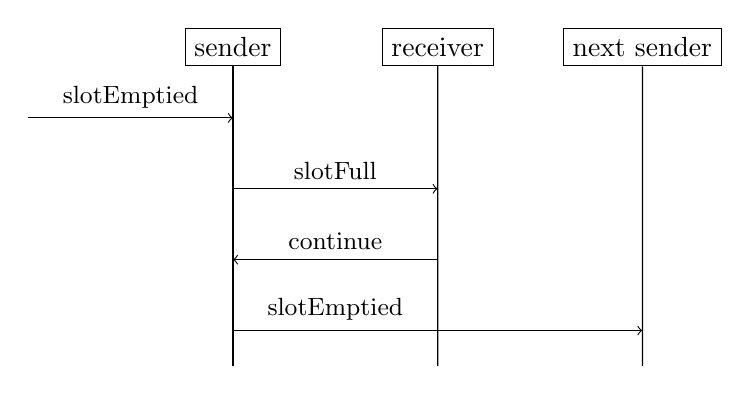
\begin{tikzpicture}[xscale = 1.3,yscale = 0.9]
\draw (0,0) node[draw](sender){sender};
\draw (2,0) node[draw](receiver){receiver};
\draw (4,0) node[draw](sender2){next sender};
\draw (sender) -- ++ (0,-4.5);
\draw (receiver) -- ++ (0,-4.5);
\draw (sender2) -- ++ (0,-4.5);
\draw[->] (-2.0,-1) -- 
  node[above] {\small\scalastyle slotEmptied} (0,-1);
\draw[->] (0,-2) -- node[above] { \small\scalastyle slotFull} (2,-2);
\draw[<-] (0,-3) -- node[above] { \small\scalastyle continue} (2,-3);
\draw[->] (0,-4) -- node[above, near start] {\small\scalastyle slotEmptied} (4,-4);
\end{tikzpicture}
\end{center}
\caption{Sequence diagram showing the sequence of signals in the
  semaphore-based implementation of a synchronous channel.}
\label{fig:semaphore-syncChan-SD} 
\end{figure}


%%%%%

\begin{figure}
\begin{scala}
class SemaphoreSyncChan[A] extends tacp.monitors.SyncChanT[A]{  
  /** The current or previous value. */
  private var value = null.asInstanceOf[A]

  /** A semaphore for signalling to receiver that a value has been deposited. */
  private val slotFull = new SignallingSemaphore

  /** A semaphore for signalling to current sender that it can continue. */
  private val continue = new SignallingSemaphore

  /** A semaphore for signalling to the next sender that the previous value has
    * been read. */
  private val slotEmptied = new MutexSemaphore

  /* Note: the semaphores together provide mutual exclusion. */

  def send(x: A) = {
    slotEmptied.down()      // Wait for previous value to be consumed (1).
    value = x               // Deposit my value.
    slotFull.up()           // Pass baton to receiver at (2).
    continue.down()         // Wait for receiver (3).
    slotEmptied.up()        // Pass baton to next sender at (1).
  }

  def receive(): A = {
    slotFull.down()         // Wait for sender (2).
    val result = value      // Take value.
    continue.up()           // Pass baton to current sender at (3).
    result
  }
}
\end{scala}
\caption{A synchronous channel implemented using semaphores.}
\label{fig:SemaphoreSyncChan}
\end{figure}

%%%%%

The implementation is in Figure~\ref{fig:SemaphoreSyncChan}.
The three semaphores collectively provide mutual exclusion: when any
thread is active, all semaphores are down; when no thread is active, a
single semaphore is up.  Initially, just |slotEmptied| is up.

Unlike the implementations in earlier chapters, there is no need to have an
extra |full| variable indicating that the current value is valid: the
|slotFull| and |slotEmptied| semaphores fulfil that role.


We can argue that the signals must happen in the expected order.  We write
``$\sm{slotEmptied.down}_1$'' for the first |down| performed on |slotEmptied|,
etc.  Then we can argue as follows, based on a combination of program order
for the two threads, and the fact that each |up| must precede the
corresponding |down| (except for the initial |down| on |slotEmptied|, since
that semaphore is initially in the \emph{up} state).  
\[
\begin{array}{rcl@{\qquad}l}
\sm{slotEmptied.down}_1 & \prec & \sm{slotFull.up}_1 & 
  \mbox{(program order for \SCALA{send})} \\
  & \prec & \sm{slotFull.down}_1 & \sm{(signal on {\scalashape slotFull})} \\
  & \prec & \sm{continue.up}_1 & \mbox{(program order for \SCALA{receive})} \\
  & \prec & \sm{continue.down}_1 & \sm{(signal on {\scalashape continue})} \\
  & \prec & \sm{slotEmptied.up}_1 & \mbox{(program order for \SCALA{send})} \\
  & \prec & \sm{slotEmptied.down}_2 & 
     \sm{(signal on {\scalashape slotEmptied})} \\
  & \prec & \ldots
\end{array}
\]
In particular, for each semaphore $s$,\, $s.\sm{down}_n \prec
s.\sm{up}_{n+1}$, for each~$n$, so the precondition of the |up| operation is
satisfied.

\begin{instruction}
Study the implementation, and make sure you understand why the semaphore
operations occur in the above order.
\end{instruction}

%%%%%

The signalling here is in a slightly different order from that in the
implementation using an SCL monitor in Section~\ref{sec:conditionsChan}.
There, the receiver---rather than the sender---signals to the next sender.
Figure~\ref{fig:SemaphoreSyncChan-incorrect} gives a corresponding signalling
strategy using semaphores---but it turns out that this is incorrect!

%%%%%

\begin{figure}
\begin{scala}
  def send(x: A) = {
    slotEmptied.down()       // Wait for previous value to be consumed (1).
    value = x               // Deposit my value.
    slotFull.up()             // Pass baton to receiver at (2).
    continue.down()           // Wait for receiver (3).
  }

  def receive(): A = {
    slotFull.down()           // Wait for sender (2).
    val result = value      // Take value.
    continue.up()             // Pass baton to current sender at (3).
    slotEmptied.up()          // Pass baton to next sender at (1).
    result
  }
\end{scala}
\caption{An incorrect implementation of a synchronous channel using
  semaphores.}
\label{fig:SemaphoreSyncChan-incorrect}
\end{figure}

%%%%%

With the version in Figure~\ref{fig:SemaphoreSyncChan-incorrect}, suppose a
|send| operation is suspended just before performing |continue.down()|.  Then
the current receiver can signal on |continue| and |slotEmptied|.  Then the
following sender and receiver can run, leading to a second |continue.up()|.
But thus breaks the precondition of |up|!  If our implementation of semaphores
had allowed such a second |up|, it would have been a lost signal.  The correct
implementation ensures a strict order in which critical events occur. 


%%%%%%%%%%%%%%%%%%%%%%%%%%%%%%%%%%%%%%%%%%%%%%%%%%%%%%%

\section{First-Come, First-Served Locking}
\label{sec:queueLock}

We now consider an implementation of a lock to allow threads to access a
shared resource under mutual exclusion.  However, we also want to ensure that
threads gain access in a first-come, first-served order (we will make clear
later precisely what we mean by this). 
% (Note that this will
% have a performance overhead, but might be desirable in some circumstances.)
%

Figure~\ref{fig:QueueLock} gives an implementation of such a lock, using
semaphores.  It uses a variable |busy| to record whether a thread currently
holds the lock.  If a thread is forced to wait to gain access to the resource,
it creates a new semaphore, places it in a queue, and then waits on it.  When
a thread finishes with the resource, it passes the baton to the thread waiting
on the first semaphore in the queue (if there is one) by raising that
semaphore.  The semaphore |mutex| enforces mutual exclusion on the object's
variables.

%%%%%

\begin{figure}
\begin{scala}
class QueueLock extends LockT{
  /** A queue of semaphores for waiting threads. */
  private val queue = new scala.collection.mutable.Queue[Semaphore]

  /** Is the resource busy? */
  private var busy = false

  /** Semaphore for mutual exclusion on this object's variables. */
  private val mutex = new MutexSemaphore

  /** Acquire the lock. */
  def acquire() = {
    mutex.down()
    if(busy || !queue.isEmpty){ // Thread has to wait.
      val sem = new SignallingSemaphore
      queue.enqueue(sem)
      mutex.up(); sem.down() // Wait for turn.
      assert(!busy)  
    }
    busy = true
    mutex.up()
  }

  /** Release the lock. */
  def release() = {
    mutex.down()
    busy = false
    if(queue.nonEmpty){ // Signal to next thread in £queue£.
      val first = queue.dequeue(); first.up()
    }
    else mutex.up()
  } 
}
\end{scala}
\caption{A lock providing first-come, first served access.}
\label{fig:QueueLock}
\end{figure}

%%%%%

\begin{instruction}
Study the details of the lock.
\end{instruction}

Threads that are forced to wait subsequently acquire the lock in the order in
which they add their semaphores to the queue.  This means that threads acquire
the lock in the order in which they acquire the |mutex| semaphore.  It is
reasonable to assume that threads use the resource protected by the lock for a
reasonable amount of time, normally longer than the time they spend running in
the |acquire| operation; thus the resource itself is the main bottleneck,
rather than the lock.  Thus if thread~$t_1$ calls |acquire| a reasonable time
before thread~$t_2$, we can expect $t_1$ to acquire the lock first.

We define the \emph{doorway period} to be the period during which a thread
registers its desire to acquire the lock, placing its semaphore in the queue
if necessary.  We can expect this period to be quite short.  By contrast, the
\emph{waiting period}, where a thread waits to receive a signal on its
semaphore, might be rather longer.  Our first-come, first-served property is
that if thread~$t_1$ completes its doorway period before~$t_2$, then $t_1$
will access the resource first.


This technique---where each thread creates a semaphore, stores it, and then
waits on it---can be used in a number of scenarios to allow the current
thread to selectively pass the baton to a particular thread.
%% : each thread that
%% has to wait, creates a new semaphore, stores it, and waits on it.
%
Sometimes it is necessary to store some extra information with each such
semaphore, so that the current thread can choose between the waiting threads.
This choice should be made so that the thread that receives the signal can
then do something useful. 

